A general method of calculating the rate constant of two particles with a given potential, finding the collisional cross section, which is then averaged over a velocity distribution to find the rate constant.\cite{Zhang2017,Brouard2012} The interaction potential of two reactants is generally defined as
\begin{equation}
    V(r) = \sum_n - \frac{C_n}{r^n}
\end{equation}
where $C_n$ is the interaction coefficient of order $n$. We may write the effective potential in the center of mass frame as
\begin{equation}
    V_{\mathrm{eff}} = \frac{l^2}{2 \mu_R r^2} + V(r)\label{eq: veff}
\end{equation}
where $\mu_R=m_1 m_2/(m_1 + m_2)$ is the reduced mass of the two particles. The competition between the repulsive and attractive terms creates a barrier as seen in Figure \ref{fig: veff}.
\begin{figure}[H]
	\centering
	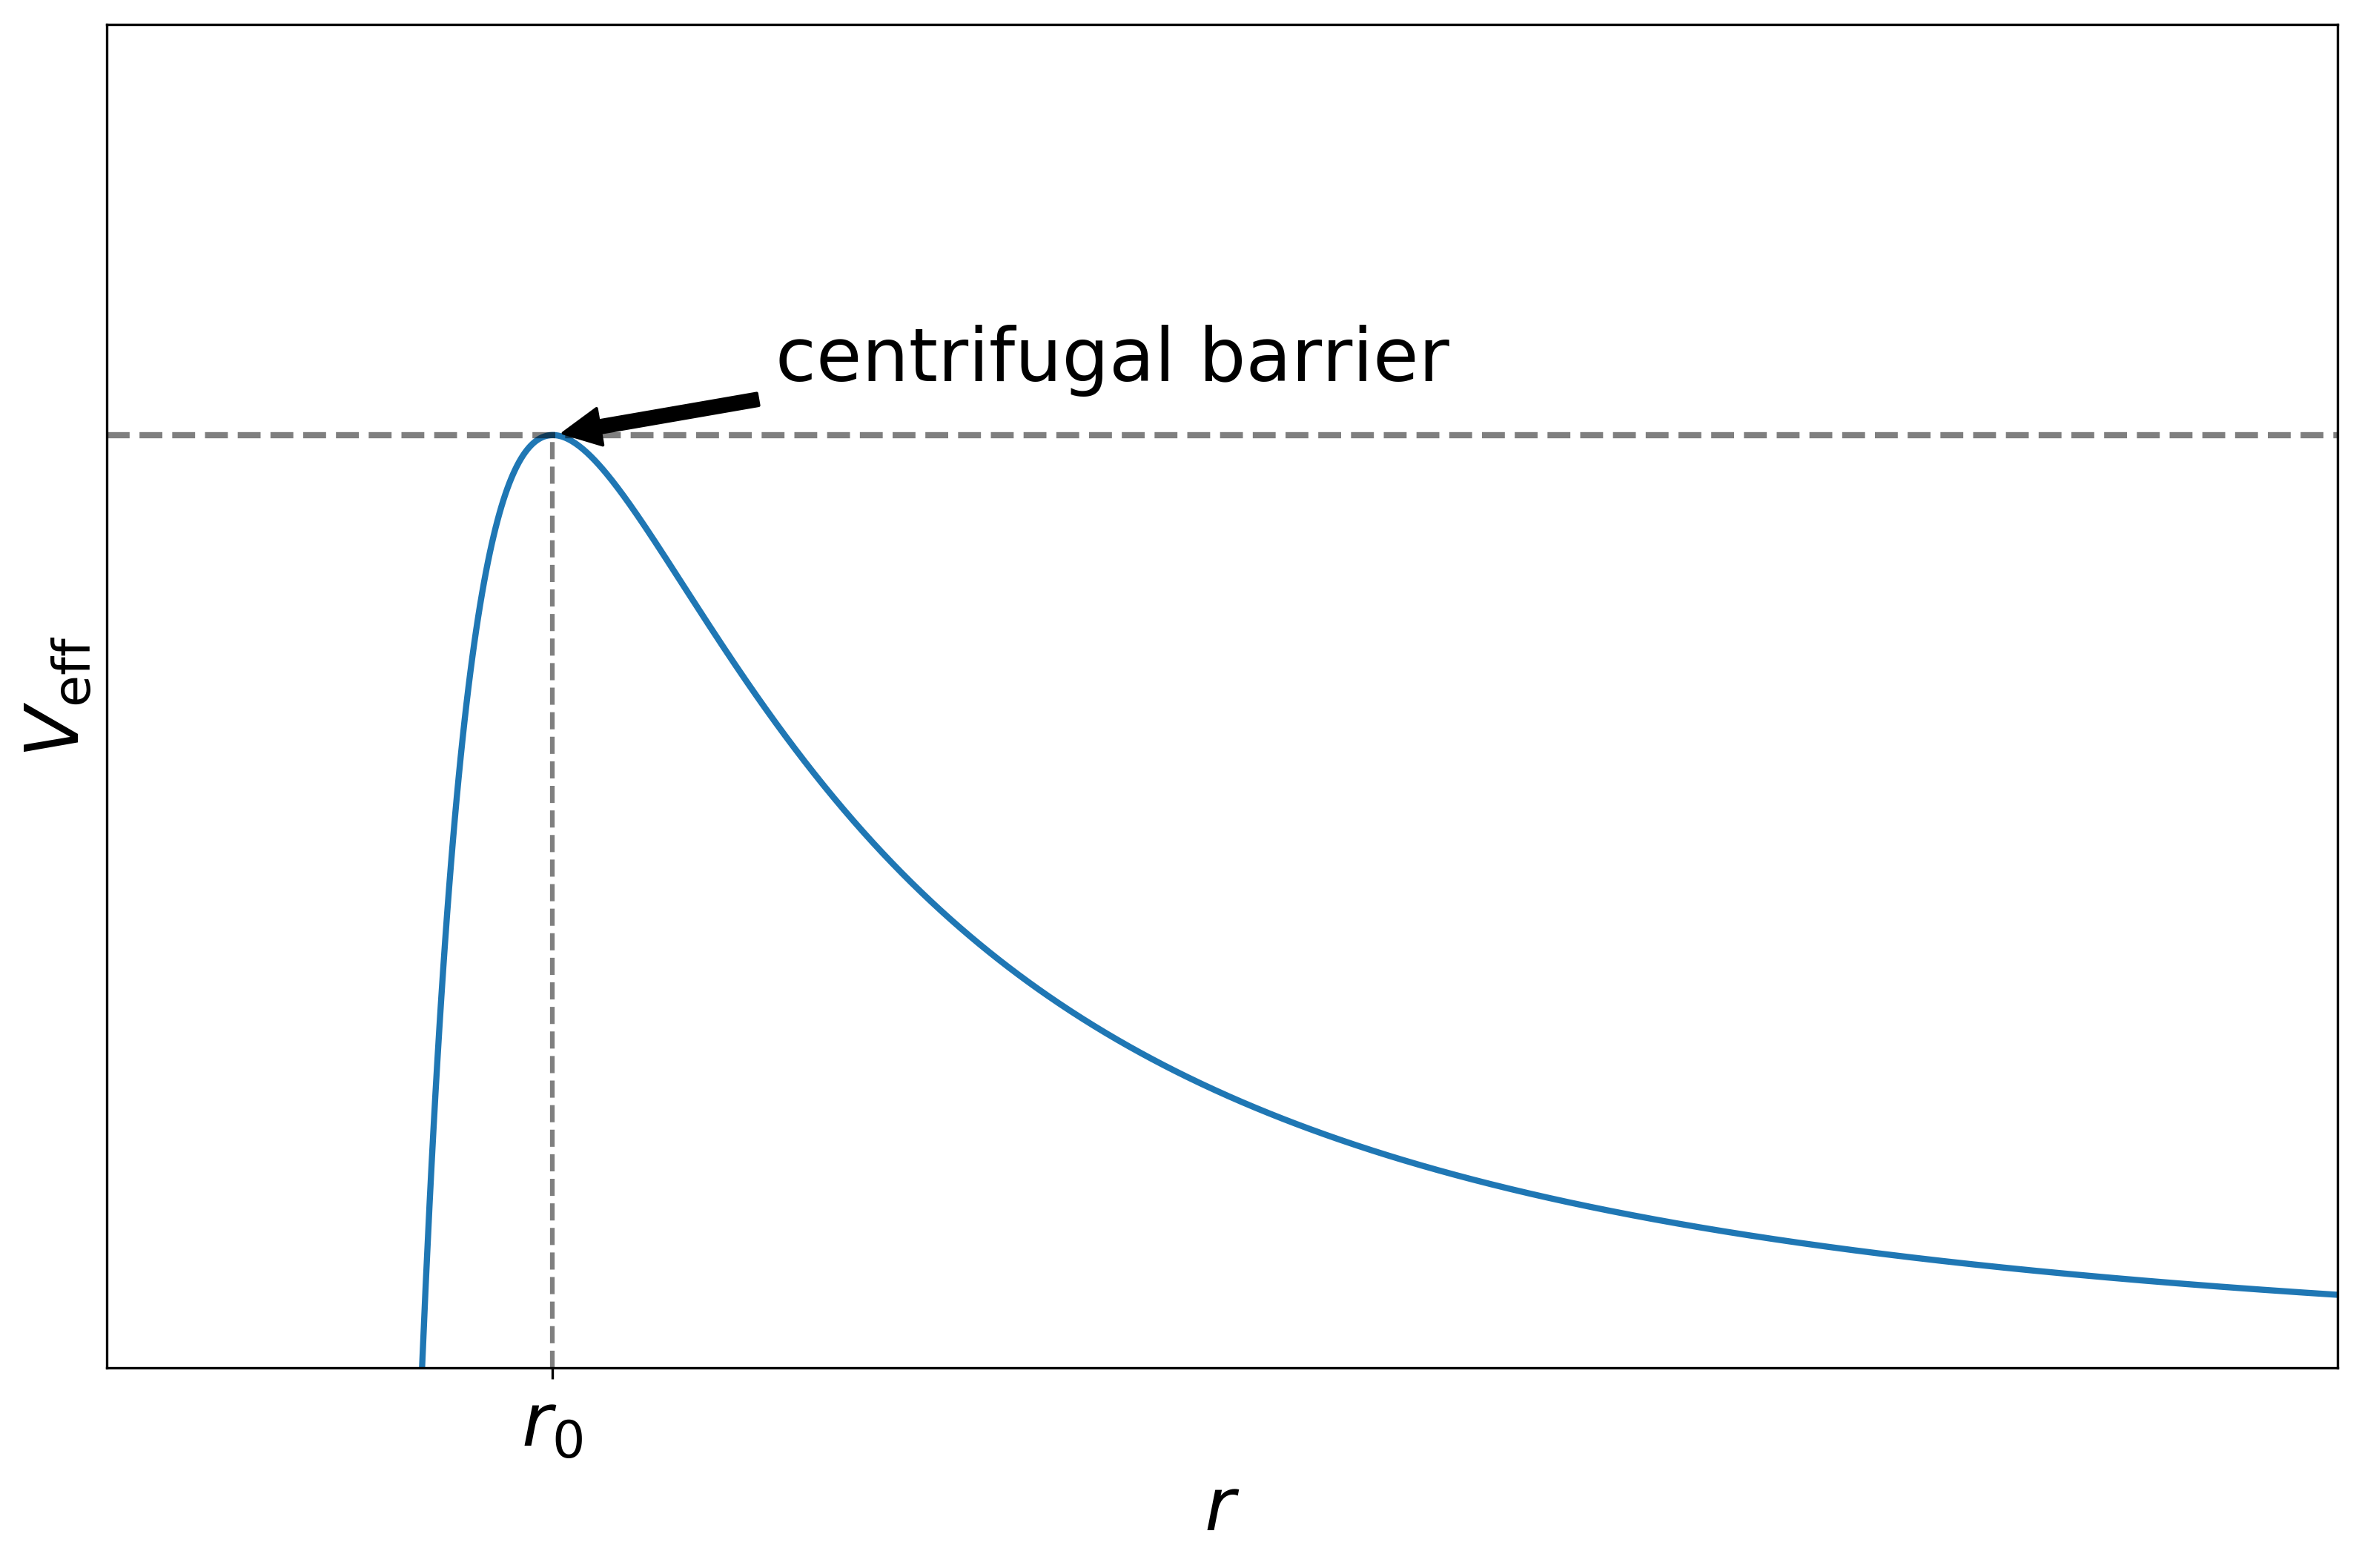
\includegraphics[width=0.8\textwidth]{images/v_eff.png}
	\caption{An arbitrary effective potential of an monopole-induced-dipole interaction. The maximum of the potential at $r_0$ creates a centrifugal barrier. Only particles with $E_{\mathrm{col}} > V_{\mathrm{eff}}$ surmount the barrier and collide.}
	\label{fig: veff}
\end{figure}
To find the condition for a collision to occur, we first find the position $r_0$ corresponding to the maximum of the effective potential, which is the value of the centrifugal barrier.
\begin{align*}
    \frac{\partial V_{\mathrm{eff}}}{\partial r}\bigg|_{r_0} & = 0 \\
    \therefore r_0 & = \left(\frac{n \mu_R C_n}{l^2}\right)^{1/n-2}
\end{align*}
Substituting $r_0$ back into equation $\ref{eq: veff}$, we find the maximal value of the effective potential:
\begin{equation}
    V_{\mathrm{eff}}(r_0) = \left(\frac{l^2}{\mu_R}\right)^{\frac{n}{n-2}} \frac{n-2}{2n}(n C_n)^{-\frac{2}{n-2}}
\end{equation}
This then defines the energy necessary for a collision, for if $E_{\mathrm{col}}$ exceeds $V_{\mathrm{eff}}(r_0)$, the reactants will be able to surmount the centrifugal barrier and collide. For the condition where $V_{\mathrm{eff}}(r_0) = E_{\mathrm{col}} = \frac{1}{2}\mu_R v^2$, we define the maximum value for the angular momentum $l$ and the impact parameter $b$.
\begin{align*}
    l_{\max} & = (\mu_R n)^{1/2}(C_n)^{1/n} \left(\frac{2 E_{col}}{n-2}\right)^{\frac{n-2}{2n}} \\
    b_{\max} & = \frac{l_{\max}}{\mu_R v}
\end{align*}
We can then define a collision cross section dependent on the collision energy:
\begin{align*}
    \sigma(E_{col}) & = \pi b^2_{\max} \\
    & = \frac{\pi}{2} n \left(\frac{2}{n-2}\right)^{\frac{n-2}{2}} \left(\frac{C_n}{E_{col}}\right)^{\frac{2}{n}}
\end{align*}
Integrating the collision cross section with a Maxwell Boltzmann distribution yields a generalized rate constant as a function of temperature and $n$.
\begin{align}
    k(T) & = \int_0^{\infty} v f(v) \sigma(v) dv \label{eq: k int} \\
    & = \sqrt{\frac{2 \pi}{\mu_R}}n\left(\frac{2}{n-2}\right)^{\frac{n-2}{2}}C_n^{2/n}(k_B T)^{\frac{n-4}{2n}}\Gamma\left(2-\frac{2}{n}\right) \label{eq: k(T)}
\end{align}
For instance, the monopole-induced-dipole potential of order $n=4$ has the form and rate constant
\begin{align}
	V_L & = -\frac{\alpha q^2}{2r^4} \label{eq: V_L} \\
	k(T) & = 2\pi q \sqrt{\frac{\alpha}{\mu_R}} \label{eq: k langevin}
\end{align}
where $\alpha$ is the polarizability of the neutral reactant, and $q$ is the monopole charge. The corresponding $k(T)$ in equation \ref{eq: k langevin} is known as the Langevin rate constant, which is famously temperature independent.